\chapter{Technische Informationen}
\label{ch:TechnischeInfos}

\newcommand*{\checkbox}{{\fboxsep 1pt%
\framebox[1.30\height]{\vphantom{M}\checkmark}}}

\section{Aktuelle Dateiversionen}

\begin{center}
\begin{tabular}{|l|l|}
\hline
Datum & Datei \\
\hline\hline
\htldiplDate & \texttt{thldipl} \\
\hline
\htlDate       & \texttt{htl.sty} \\
\hline
\end{tabular}
\end{center}




\section{Details zur aktuellen Version}


Das ist eine völlig überarbeitete Version der Vorlage, die \texttt{pdf\-latex}
"`native"' und nicht (wie bisher) im DVI-Kompatibiliätsmodus verwendet. 
Der primäre Anlass für diesen Schritt war die Frage, wie man automatisch Metadaten im PDF-File ablegen kann, 
woraus sich allerdings eine Fülle von Änderungen ergeben haben, die in Summe die Arbeit mit LaTeX um 
Einiges leichter machen sollten. 

Es wird nunmehr als Ausgabe \emph{direkt} PDF erzeugt und (normalerweise) keine DVI-Datei mehr.
Der "`klassische"' DVI-PS-PDF-Modus ist allerdings weiterhin verfügbar (und auch notwendig, 
wenn man mit \texttt{psfrag} arbeiten möchte oder muss).

\subsubsection*{Verwendung unter Linux}
Was muss ich tun, um diese Version für meine Arbeit zu verwenden:
\begin{enumerate}
  \item Die Packete \textbf{texlive} und \textbf{texlive-lang-german} müssen
  installiert sein.
  \item \textbf{Eclipse} mit der Erweiterung \textbf{Texlipse} oder ein anderes
  \latex Frontend sollte installiert sein.
  \item Die Dateien \texttt{htldipl.cls} und \texttt{htl.sty} sind in das eigene
  Projektverzeichnis zu kopieren.
\end{enumerate}

\subsubsection*{Verwendung unter Windows}
Was muss ich tun, um diese Version für meine Arbeit zu verwenden:
\begin{enumerate}
\item \textbf{MikTeX 2.8} oder höher muss installiert sein.
%\item \textbf{SumatraPDF}%
%\footnote{\url{http://blog.kowalczyk.info/software/sumatrapdf/}} 
%Viewer muss installiert sein.
\item Die Dateien \texttt{htldipl.cls} und \texttt{htl.sty} sind in das eigene
Arbeitsverzeichnis zu kopieren.
%\item TeXniCenter-Profile für Sumatra importieren (aus beiliegender Datei \url{_tc_output_profiles_sumatra.tco}).
\end{enumerate}

\subsubsection*{Verwendung unter Mac~OS}

Unter Mac~OS wurde die aktuelle Vorlage noch nicht getestet. Der folgende Text bezieht sich auf die alte Vorlage und ist möglicherweise nicht mehr korrekt.

Diese Version sollte insbesondere unter \emph{MacTeX} problemlos laufen.
Was ist konkret zu tun, um die aktuelle Version unter Mac~OS zu verwenden:
\begin{enumerate}
\item \emph{MacTex} (2009 oder höher) muss installiert sein.
\item Ein PDF-Viewer muss verfügbar sein (\zB\ Mac~OS \emph{Preview}) -- \emph{TeXworks} hat eine eigenständige PDF Ausgabe inkludiert.
\item Die Zeichenkodierung des Editors muss auf ISO-8859-1 (Latin 1) gestellt sein.
\item Die Dateien \texttt{htldipl.cls} und \texttt{htl.sty} sind in das eigene
Arbeitsverzeichnis zu kopieren.
\end{enumerate}

\section{Einstellungen unter Windows} 
\label{sec:EinstellungAusgabeprofile}

Die folgenden Angaben beziehen sich auf eine bewährte Arbeitsumgebung unter MS Windows (XP, Vista, Win7) mit MikTeXund TeXnicCenter, mit folgenden Installationspfaden:
%
\begin{quote}
\verb!C:\Program Files\MiKTeX 2.8\! \\
%\verb!C:\Program Files\SumatraPDF\! \\
\verb!C:\Program Files\TeXnicCenter\! 
\end{quote}
%
Falls neuere Versionen dieser Komponenten installiert sind, müssen natürlich die nachfolgend angegebenen Pfade entsprechend modifiziert werden.


\subsection{TeXnicCenter-Ausgabeprofile}
\label{sec:TeXnicCenterUndMikTeX}

TeXnicCenter definiert den Verarbeitungsablauf des LaTeX-Dokuments anhand von Ausgabeprofilen, wobei die oben genannten Komponenten als externe Programme mit entsprechenden Argumenten aufgerufen werden.
Die Einstellung der Ausgabeprofile erfolgt in TeXnicCenter über das Menü
\textsf{Ausgabe}$\rightarrow$\textsf{Ausgabeprofile definieren...} (Abb.\ \ref{fig:techniccenter-profile-latex}). 
Die Profile werden (abhängig von der installierten Software) üblicherweise beim ersten Start von TeXnicCenter durch den zugehörigen "`Wizard"' voreingestellt. 


\begin{figure}
\centering\small
\setlength{\tabcolsep}{0pt}%
\begin{tabular}{c@{~}c}
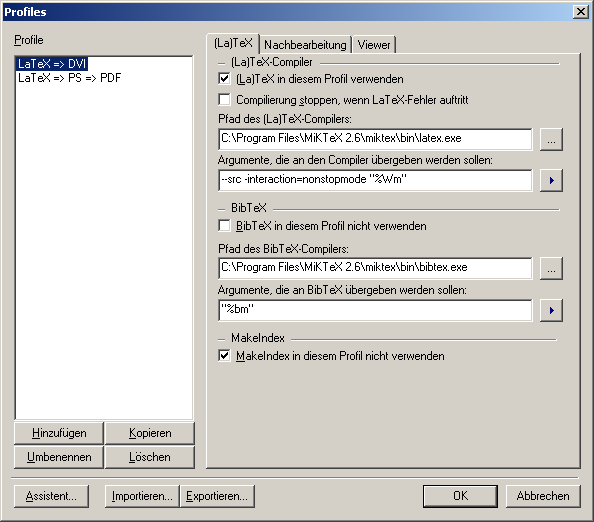
\includegraphics[width=0.49\textwidth]{techniccenter-profile-dvi-26} &
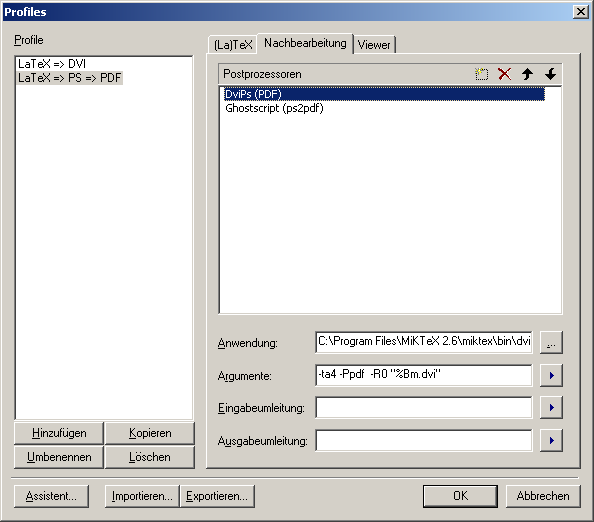
\includegraphics[width=0.49\textwidth]{techniccenter-profile-dvips-26} \\[4pt]
(a) & (b)
\end{tabular}
\caption{Spezifikation der Ausgabeprofile in TeXnicCenter.}
\label{fig:techniccenter-profile-latex}
\end{figure}

Für diese Vorlage wird die verwendung des Ausgabeprofiels \texttt{LaTeX => PDF} empfohlen.

%
%In der Datei \verb!tc_output_profiles_sumatra.tco! sind  folgende beiden "`maßgeschneiderten"' Ausgabeprofile für TexNicCenter angelegt (Import über \textsf{Build} $\rightarrow$ \textsf{Define Output Profiles ...}):
%\begin{itemize}
	%\item \verb!LaTeX => PDF (Sumatra)! -- Standard, direkte Erzeugung von PDF,
	%\item \verb!LaTeX => PS => PDF (Sumatra)! -- PDF "`klassisch"' via DVI und PS.
%\end{itemize}
%
%
%
%\subsubsection{Profil "`\texttt{LaTeX => PDF (Sumatra)}"'}
%
%Das ist das mit diesem Setup normalerweise verwendete Standardprofil.
%
%\paragraph{(La)Tex:}
%\begin{itemize}
  %\item Path to the (La)TeX compiler: \\
        %\begin{small} \verb!C:\Program Files\MiKTeX 2.8\miktex\bin\pdflatex.exe!\end{small}
  %\item Command line arguments to pass to the compiler:\\
%\begin{small}
   %\verb!-synctex=-1 -interaction=nonstopmode "%pm"!
%\end{small}
%\end{itemize}
%
%\paragraph{Postprocessor:} 
%leer, kein Postprocessor notwenig.
%
%\paragraph{Viewer:}
%\begin{itemize}
%\item Path of executable: \\
%\begin{small}
    %\verb!C:\Program Files\SumatraPDF\SumatraPDF.exe ! \\ 
    %\verb!-inverse-search "\"C:\Program Files\TeXnicCenter\TEXCNTR.EXE\" !\\
    %\verb!/ddecmd \"[goto('%f','%l')]\""!
%\end{small}
%%
%\item View project's output: \\
%\begin{small}
    %\checkbox\ Command line argument \\\
    %Command: \verb!"%bm.pdf"!
%\end{small}
%%
%\item Forward search:\\
%\begin{small}
    %\checkbox\ DDE command \\\
    %Command: \verb![ForwardSearch("%bm.pdf","%Wc",%l,0)]! \\
    %Server: \verb!SUMATRA! \\
    %Topic: \verb!Control!
%\end{small}
%\item Close document before running (La)TeX:\\
%\begin{small}
    %\checkbox\ Do not close
%\end{small}
%\end{itemize}
%
%
%
%
%\subsubsection{Profil "`\texttt{LaTeX => PS => PDF (Sumatra)}"'}
%
%Profil ausschließlich für den DVI-PS-Workflow (über DVI und PostScript).
%
%\paragraph{(La)Tex:}
%\begin{itemize}
  %\item Path to the (La)TeX compiler: \\
        %\begin{small} \verb!C:\Program Files\MiKTeX 2.8\miktex\bin\latex.exe!\end{small}
  %\item Command line arguments to pass to the compiler:\\
%\begin{small}
   %\verb!-synctex=-1 -interaction=nonstopmode "%pm"!
%\end{small}
%\end{itemize}
%
%\paragraph{Postprocessor:}
%\begin{itemize}
  %\item DviPS (PDF): \\
        %\begin{small} 
        %Executable: \verb!C:\Program Files\MiKTeX 2.8\miktex\bin\dvips.exe! \\
        %Arguments: \verb!-ta4 -P pdf -R0 "%Bm.dvi"!
        %\end{small}
  %\item Ghostscript (ps2pdf):\\
  		%\begin{small} 
        %Executable: \verb!C:\Program Files\gs\gs8.64\bin\gswin32c.exe! \\
        %Arguments: \verb!-q -dPDFSETTINGS=/prepress -sPAPERSIZE=a4 -dSAFER! \\
         %\verb!-dBATCH -dNOPAUSE -sDEVICE=pdfwrite -sOutputFile="%bm.pdf"! \\
         %\verb!-c save pop -f "%bm.ps"!
      %\end{small}
%\end{itemize}
%
%\paragraph{Viewer:}
%wie in Profil A. (\texttt{LaTeX => PDF (Sumatra)}).
